\documentclass{school-22.211-notes}
\date{April 30, 2012}

\begin{document}
\maketitle

\lecture{Point Kinetics With Feedbacks} \label{PKE-with-feedback}
Why we care about feedbacks? 
\begin{enumerate}
\item It used to be that we assume an artificially high rod worth and model fuels fresh. Then people realize that, the rod movement in one assembly changes the local flux distribution as illustrated in Fig.~\ref{local-flux-changes}. 
  \begin{figure}[ht]
    \centering
    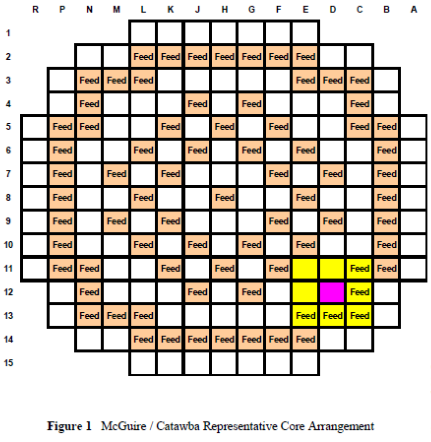
\includegraphics[width=2in]{images/pke/local-flux-changes.png}
    \caption{Local Flux Changes} \label{local-flux-changes}
  \end{figure}

\item If we perform a rod ejection at hot zero power, the magnitude of flux/power can change from a few Watt to 20,000 MW in less than 1s! Also the fuel enthalpy at failure is dependent on fuel BU (the higher the BU, the easier it is for the fuel to fail) as in Fig.~\ref{failure-depend-on-BU}. Thus we need to model control rods somewhat faithfully to get a reasonable safety analysis. 
  \begin{figure}[ht]
    \centering
    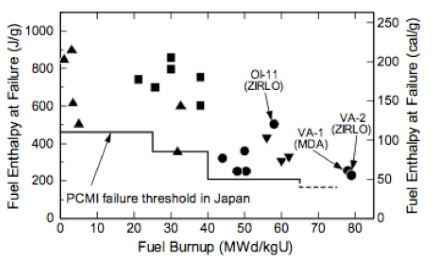
\includegraphics[width=4in]{images/pke/failure-depend-on-BU.png}
    \caption{Fuel Enthalpy at Failure Depends on Fuel BU} \label{failure-depend-on-BU}
  \end{figure}

\item The importance of modeling feedback can be illustrated in Fig.~\ref{feedback}. Without feedback, the reactor wants to be a bomb and the power shoots up with an asymptotic period. With Doppler feedback, both the reactivity and the power decreases before the rod is even fully inserted. When correctly designed, reactors use feedback effects to keep them from acting like bombs\footnote{There is no Doppler feedback for fast reactors, so fast reactors have to do all kind of tricks to get a negative feedback. Also fast reactors have positive sodium void worth, because as energy deposits in the sodium, voids are generated, pushing sodium away, generating a positive sodium void worth}. The feedback is especially strong when $\rho > 1$\$. \textbf{A second peak is the characteristic of longer rod change.} 
\end{enumerate} 
  \begin{figure}[ht]
    \centering
    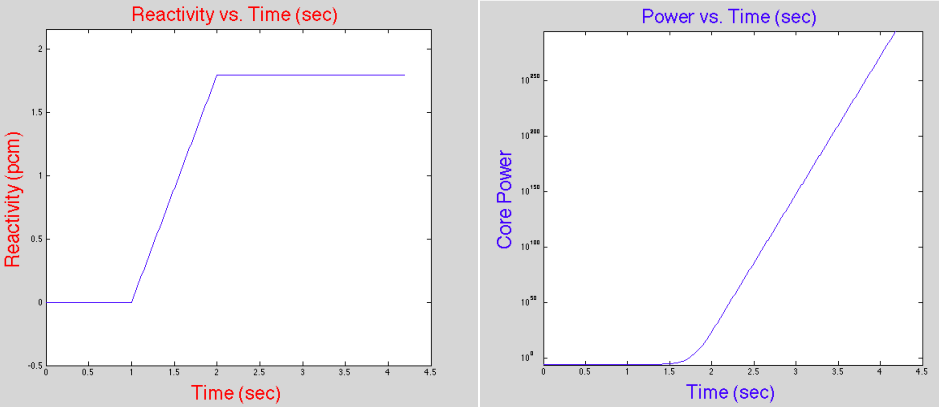
\includegraphics[width=6in]{images/pke/feedback1.png}
    \\
    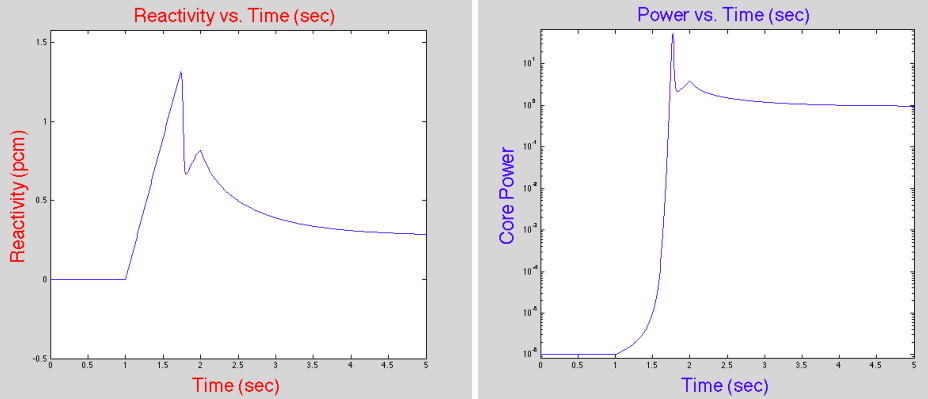
\includegraphics[width=6in]{images/pke/feedback2.png}
    \caption{1.5\$ RIA Without Feedback (top row) and With Doppler Feedback (bottom row)}\label{feedback}
  \end{figure}



\clearpage
\topic{Fuchs-Nordheim Model}
The Fuchs-Nordheim Model predicts the shape and the magnitude of the transient. We do not really solve the analytical solution of this model, but instead study some characteristics from it. 

\subtopic{Assumptions}
To start, we make three assumptions\footnote{The historical reason for these assumptions is that the model was developed for weapon use, hence $\rho \gg \beta$ and rapid transient.}, 
\begin{enumerate}
\item If $\rho \gg \beta$, we can ignore the delayed neutrons, hence the precursor equation in PKEs goes away, and we are left with the power distribution $P(t)$ with no precursor term\footnote{we use $P(t)$ instead of $T(t)$ for the shape function now to avoid the confusion with temperature $T$ that we would use repeatively in this section.}. 
  \eqn{ \ddt P(t) &= \frac{\rho(t) - \beta}{\Lambda} P(t) + \Sum_i \lambda_i C_i (t) \approx \frac{\rho(t) - \beta}{\Lambda} P(t) \label{fn-eq1}}
  It is fair to ignore the precursors, because as in Fig.~\ref{fn1} top row, we can see that the power with precursor is small enough that the F-N model provides a good approximation; the bottom row images are plotted on a log-log scale to show the small difference made by the precursors.  
\begin{figure}[ht]
  \centering
  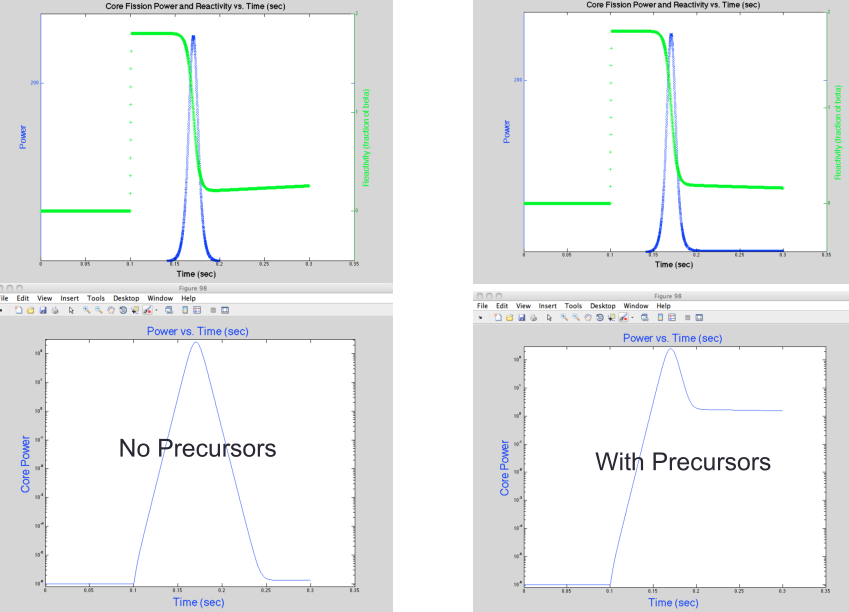
\includegraphics[width=6in]{images/pke/fn1.png}
  \caption{Assumption in Fuchs-Nordheim: No Precursors}\label{fn1}
\end{figure}

\item If transient is so rapid that no heat is transferred from the fuel\footnote{The time constant for heat to be removed from \ce{UO_2} fuel is about 5 mins.}, 
  \eqn{ T_{\mathrm{fuel}} = T_{\mathrm{fuel}}^0 + \frac{1}{C_p} \int P(t) \dt \label{fn-eq2} }

\item Assume a Doppler feedback coefficient independent of temperature (recall that we calculate that PWRs have a Doppler coefficient is abou -3 pcm/K), 
  \eqn{ \rho(t) = \rho_{\mathrm{rod}} - \alpha (T_{\mathrm{fuel}} - T_{\mathrm{fuel}}^0) \label{fn-eq3} }
\end{enumerate}

\subtopic{First Derivation}
So we want solve the first order ODE in Eq.~\ref{fn-eq1} by using Eq.~\ref{fn-eq2} and \ref{fn-eq3}. We differentiate Eq.~\ref{fn-eq2} to get,
\eqn{ \frac{\dT_{\mathrm{fuel}} (t)}{\dt} = \frac{P(t)}{C_p} \label{fn-eq4}}
Plug Eq.~\ref{fn-eq3} into Eq.~\ref{fn-eq1} (omitting $T_{\mathrm{fuel}}^0$), 
\eqn{ \frac{\dP(t)}{\dt} = \frac{\rho_{\mathrm{rod}} - \alpha T_{\mathrm{fuel}} - \beta}{\Lambda} P(t) \label{fn-eq5} }
Divide Eq.~\ref{fn-eq5} by \ref{fn-eq4}, then integrate, 
\begin{align}
\frac{\dP(t)}{\dT_{\mathrm{fuel}}} &= \frac{\dP(t)}{\dt} \bigg/  \frac{\dT_{\mathrm{fuel}} (t)}{\dt} =  \frac{(\rho_{\mathrm{rod}} - \alpha T_{\mathrm{fuel}} - \beta ) C_p}{\Lambda} 
= \frac{1}{\Lambda} \left[ C_p (\rho_{\mathrm{rod}} - \beta) - \alpha C_p T_{\mathrm{fuel}} \right] \\
\Aboxed{ P(t) &= P_0 + \frac{1}{\Lambda} \left[ C_p (\rho_{\mathrm{rod}} - \beta) T_{\mathrm{fuel}} (t)  - \frac{\alpha C_p}{2} T^2_{\mathrm{fuel}} (t) \right]  } \label{fn-power}
\end{align}
Eq.~\ref{fn-power} can be used to find peak power behavior, that is, we set $\frac{\dP}{dT_{\mathrm{fuel}}} = 0$, 
\eqn{ \frac{1}{\Lambda} \left[ C_p (\rho_{\mathrm{rod}} - \beta) - \alpha C_p T_{\mathrm{fuel}}^{\mathrm{peak}} \right] &= 0 }
\eqn{ \Aboxed{ T_{\mathrm{fuel}}^{\mathrm{peak}} &= \frac{\rho_{\mathrm{rod}} - \beta}{\alpha} } \label{fn-11} }
Then we can solve for peak power as well, 
\eqn{ P^{\mathrm{peak}} &= P_0 + \frac{1}{\Lambda} \left[ C_p (\rho_{\mathrm{rod}} - \beta) \frac{\rho_{\mathrm{rod}} - \beta}{\alpha}  - \frac{\alpha C_p}{2} \left( \frac{\rho_{\mathrm{rod}} - \beta}{\alpha} \right)^2 \right] }
\eqn{ \Aboxed{ P^{\mathrm{peak}} &= P_0 + \frac{C_p (\rho_{\mathrm{rod}} - \beta)^2}{2 \Lambda \alpha}}  }
Take-away Messages: 
\begin{enumerate}
\item \hi{Peak temperature is independent of neutron lifetime $\Gamma$ and heat capacity $C_p$.} 
\item Peak power is proportional to heat capacity $C_p$ and inversely proportional to prompt neutron lifetime $\Lambda$ and Doppler feedback coefficient $\alpha$. A direct consequence is, fast reactors whose $\Lambda$ is orders of magnitude smaller than LWRs are going to generate a lot of heat in a short amount of time. 
\item These equations are derived with $\rho > \beta$. As $\rho \to \beta$, the peak temperature and power become very sensitive to $\rho$. 
\end{enumerate}


\subtopic{Second Derivation}
Alternatively, we derive and integrate $P(t)$'s dependency on $\rho(t)$ instead of $T_{\mathrm{fuel}}(t)$. We use $\frac{\dP}{\dt}$ expression from the PKEs as in Eq.~\ref{fn-eq1}, and $\frac{\drho}{\dt}$ expression from Eq.~\ref{fn-power} that we derived, 
\begin{align}
\frac{\dP(t)}{\dt} &= \frac{\dP(t)}{\drho} \frac{\drho}{\dt}  \\
\frac{\dP(t)}{\drho} &=  \frac{\dP(t)}{\dt} \bigg/  \frac{\drho}{\dt}  
=   \left( \frac{\rho(t) - \beta}{\Lambda} P(t) \right) \bigg/ \left( \frac{-\alpha}{\Lambda C_p } P(t) \right) \\
&= - \frac{C_p}{\alpha} \left[ \rho(t) - \beta \right] 
\end{align}
We integrate with repsect to $\rho$ and evaluate the constant of integration by using the step reactivity $\rho_{\mathrm{rod}}$, 
\eqn{ P(t) = P_0 + \frac{C_p}{2\alpha} \left[ - (\rho(t) - \beta)^2 + (\rho_{\mathrm{rod}} - \beta)^2 \right]  }
Consider the transient terminated when $P(t)$ returns to $P_0$, then 
\eqn{ \rho_{\mathrm{end}} = 2 \beta - \rho_{\mathrm{rod}} }
Using the constant fuel temperature feedback coefficient, or Eq.~\ref{fn-eq2}, 
\eqn{ 2 \beta - \rho_{\mathrm{rod}}  = \rho_{\mathrm{rod}} - \alpha (T_{\mathrm{fuel}}^{\mathrm{end}} - T_{\mathrm{fuel}}^0 ) }
That is, 
\eqn{ \Aboxed{ T_{\mathrm{fuel}}^{\mathrm{end}} &= \frac{2 (\rho_{\mathrm{rod}} - \beta)}{\alpha} + T_{\mathrm{fuel}}^0 } }
  Compare $T_{\mathrm{fuel}}^{\mathrm{end}}$ in the above expression with $T_{\mathrm{fuel}}^{\mathrm{peak}}$ in Eq.~\ref{fn-11}, \hi{ $\Delta T_{\mathrm{fuel}}^{\mathrm{end}} = 2 \Delta T_{\mathrm{fuel}}^{\mathrm{peak}}$, where peak is when the power peaks} as in Fig.~\ref{FN2-plots}. Temperature changes independent of neutron lifetime and heat capacity again. This makes sense because we assume the transient stops when $P(t) = P_0$, and with a power distribution symmetric in time, it makes sense that the temperature rise from $P_0$ to $P^{\mathrm{peak}}$ and the temperature rise from $P^{\mathrm{peak}}$ to $P_0$ should be the same. 
\begin{figure}[ht]
  \centering
  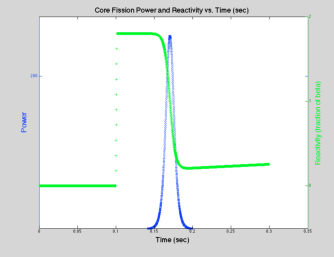
\includegraphics[width=2.6in]{images/pke/FN2-plot1.png}
  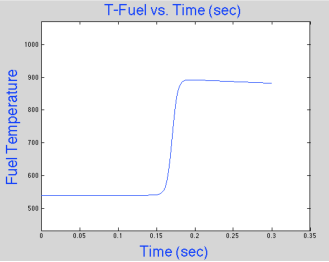
\includegraphics[width=2.5in]{images/pke/FN2-plot2.png}
  \caption{Temperature Changes in a Transient} \label{FN2-plots}
\end{figure}


\clearpage
\subtopic{Asymptotic Temperature Independent of Insertion Rate}
 \hi{Asymptotic fuel temperature is independent of the reactivity insertion rate} as in Fig.~\ref{fn2}. The power vs. time shape changes with different reactivity insertion rate, as we can see from the top row of the plots (for 2s, there is a second peak that happens when the rod is fully inserted). 

F-N model provides pretty good estimation, because temperature is basically integrated power, and the reactivity insertion rate does not matter much because we are integrating over time. Another way to think about is that there has to be something to balance out the reactivity change, and it is the Doppler feedback/temperature change that balance out the reactivity change. Thus the asymptotic temperature only depends on the asymptotic reactivity. So we can calculate, for this case for instance, 
\eqn{ T_{\mathrm{fuel}}^{\mathrm{end}}  = \frac{2 (\rho_{\mathrm{rod}} - \beta)}{\alpha} + T_{\mathrm{fuel}}^0 = \frac{2 (1.8 \times 0.0066 - 0.0066)}{3 \times 10^{-5}} + 540 = 892 \K }

  \begin{figure}[ht] 
    \centering
    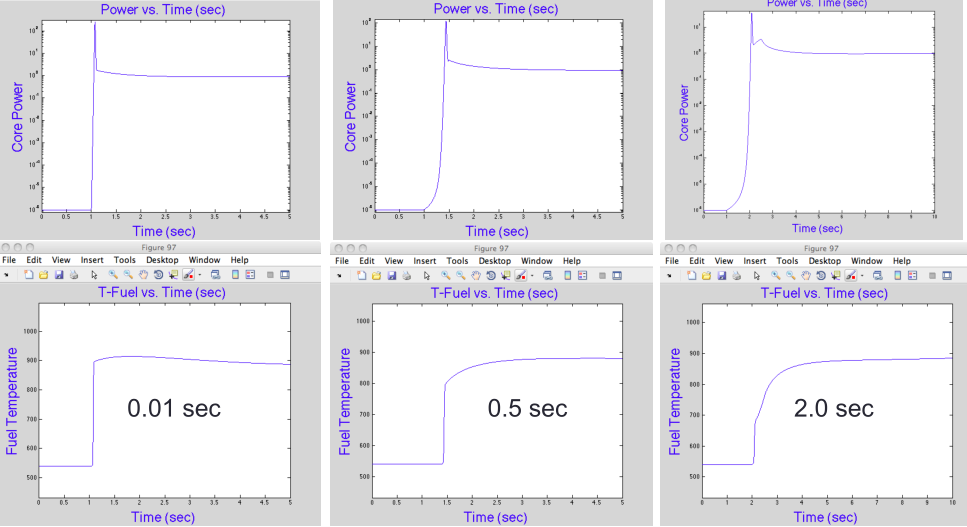
\includegraphics[width=7in]{images/pke/fn2.png}
    \caption{Fuel Temperature Independent Reactivity Insertion Rate} \label{fn2}
  \end{figure}




%%%%%%%%%%%%%%%%%%%%% PKE with Feedback!!!! %%%%%%%%%%%%%%%%%
\clearpage
\topic{PKEs with Simple Feedback}
Now we turn away from Fuchs-Nordheim model and consider the PKEs with the simplest heat conduction and transport for feedback. We have two first order ODEs, one for $T_{\mathrm{fuel}}$, one for $T_{\mathrm{coolant}}$. Basically the fuel temperature is driven by the power and conducting to the coolant. The coolant temperature is driven by the temperature different between fuel and coolant (hence fuel temperature's sink) and conducting to the inlet. 
\begin{align}
\ddt T_{\mathrm{fuel}} (t) &= a P(t) - b [T_{\mathrm{fuel}}(t) - T_{\mathrm{coolant}}(t)] \\
\ddt T_{\mathrm{coolant}} (t) &= c [T_{\mathrm{fuel}}(t) - T_{\mathrm{coolant}} (t) ] - d [T_{\mathrm{coolant}} (t) - T_{\mathrm{inlet}} (t) ] 
\end{align}
Re-write in a matrix form, 
\begin{align}
\ddt \left[ \begin{array}{c} T_{\mathrm{fuel}}(t) \\ T_{\mathrm{coolant}} (t) \end{array} \right]
+ \left[ \begin{array}{cc} b & -b \\ -c & c+d \end{array} \right] 
\left[ \begin{array}{c} T_{\mathrm{fuel}} (t) \\ T_{\mathrm{coolant}} (t) \end{array} \right] 
= 
\left[ \begin{array}{c} a P_{\mathrm{fuel}}(t) \\ d T_{\mathrm{inlet}}(t) \end{array} \right]
\end{align}
Using integrating factors to solve the above first order ODE system (we solved the exact form of problem $\ddT C + A C = Y$ for the IK equations as in Section~\ref{derivation-of-IK}),  we get (assuming zero initial power, zero initial inlet temperature), 
\begin{align}
 \left[ \begin{array}{c} T_{\mathrm{fuel}}^{n+1} \\ T_{\mathrm{coolant}}^{n+1} \end{array} \right]
&= \exp \left\{ -  \left[ \begin{array}{cc} b & -b \\ -c & c+d \end{array} \right] \Delta_t^n \right\}
\left[ \begin{array}{c} T_{\mathrm{fuel}}^n \\ T_{\mathrm{coolant}}^n \end{array} \right] \notag \\
&+ \exp \left\{ -  \left[ \begin{array}{cc} b & -b \\ -c & c+d \end{array} \right] \Delta_t^n \right\}
\left[ \begin{array}{cc} b & -b \\ -c & c+d \end{array} \right]^{-1}
\exp \left\{ \left[ \begin{array}{cc} b & -b \\ -c & c+d \end{array} \right] \Delta_t^n \right\}
\left[ \begin{array}{c} a P_{\mathrm{fuel}}^{n+1} \\ d T_{\mathrm{inlet}}^{n+1} \end{array} \right] \label{TH-analytical}
\end{align}
We make use of that we know at full power,  flow rate is 30 W/g, $C_p = 300$J/kg-s, $\alpha = -3$ pcm/K, $V_{\mathrm{coolant}} = 2 \m/\s, T_{\mathrm{inlet}}^0 = 540 \K, T_{\mathrm{coolant}}^0 = 560 \K, T_{\mathrm{fuel}}^0 = 900 \K$, core height is 4m. 

$c$ is the heat transfer coefficient, and $d$ is the axial transport term. 

%%%%%%%%%%%%%%%%
If we do not have heat transfer (axial or radial), then the fuel temperature/power would keep increasing instead of decrease slightly in p.13 Lec11. 


\clearpage
\topic{Solving the PKEs with Feedback}
We have two parts to deal with: neutronics, and TH. 

Neutronics: recall that we can write the coupled PKEs (prompt and precursor coupled) into matrix form 
\begin{align}
N &= \left[ \begin{array}{c} P \\ C_1 \\ C_2 \\ C_3 \\ C_4 \\ C_5 \\ C_6 \end{array} \right]  
& \ddt [N(t)] &= \left[ \begin{array}{ccccccc}
\frac{\rho(t) - \beta}{\Lambda} & \lambda_1  & \lambda_2 & \lambda_3 & \lambda_4 & \lambda_5 & \lambda_6 \\ 
\frac{\beta_1}{\Lambda}         & - \lambda_1 &          &           &           &           & \\
\frac{\beta_2}{\Lambda}         &             & -\lambda_2 &         &           &           & \\
\frac{\beta_3}{\Lambda}         &             &            & -\lambda_3 &        &           & \\
\frac{\beta_4}{\Lambda}         &             &           &          & - \lambda_4 &         & \\
\frac{\beta_5}{\Lambda}         &             &           &          &           & -\lambda_5 & \\
\frac{\beta_6}{\Lambda}         &             &           &          &           &           & - \lambda_6 \\
\end{array} \right] [N(t)]
\end{align}
We know the analytical solution is, 
\begin{align}
N^{n+1}  &= \exp \left\{ \left[ \begin{array}{ccccccc}
\frac{\rho(t) - \beta}{\Lambda} & \lambda_1  & \lambda_2 & \lambda_3 & \lambda_4 & \lambda_5 & \lambda_6 \\ 
\frac{\beta_1}{\Lambda}         & - \lambda_1 &          &           &           &           & \\
\frac{\beta_2}{\Lambda}         &             & -\lambda_2 &         &           &           & \\
\frac{\beta_3}{\Lambda}         &             &            & -\lambda_3 &        &           & \\
\frac{\beta_4}{\Lambda}         &             &           &          & - \lambda_4 &         & \\
\frac{\beta_5}{\Lambda}         &             &           &          &           & -\lambda_5 & \\
\frac{\beta_6}{\Lambda}         &             &           &          &           &           & - \lambda_6 \\
\end{array} \right]  \Delta_t \right\}  [N(t)]^n  \label{n-analytical}
\end{align}

TH: we have derived the analytical solution Eq.~\ref{TH-analytical}.


\subtopic{Operator Split Matrix Solution}
We evaluate the neutronics part using Eq.~\ref{n-analytical}, then plug the $P_{\mathrm{fuel}}^{n+1}$ into the TH Eq.~\ref{TH-analytical}, then plug the resolved $T_{\mathrm{fuel}}$ to update $\rho(t) = \rho_{\mathrm{rod}} - \alpha (T_{\mathrm{fuel}} - T_{\mathrm{fuel}}^0)$ in the neutronics equation. Repeat for the next time step. 

Alternatively we can do the TH part first and then neutronics. The order matters to some degree: if power is increasing, we do the TH part first and then the neutronics part. If power is decreasing, we do neutronics portion first then TH part. 

Issue: solution requires very small time steps or synchronization iterations (e.g., another iteration?). 

\begin{figure}[ht]
  \centering
  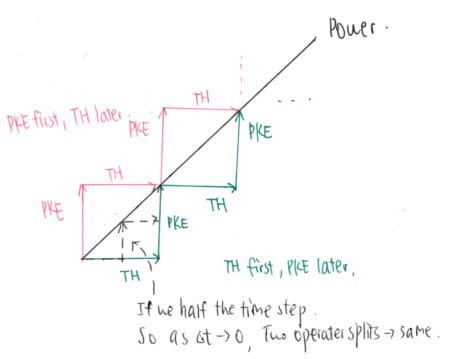
\includegraphics[width=4in]{images/methd/operator-split.png}
  \caption{Operator Splitting}
\end{figure}


[FIXME]
Take-away: 
\begin{enumerate}
\item With no synchronization step, the order of operator splits matters. 
\item With synchronization step, the two splits should approach the same. Though coarse time step with fine synchronzization step is not as good as fine time step. With a fine enough time step, it shouldn't take more than 1 iteration to synchronize. 
\end{enumerate}


 
\subtopic{Augmented Matrix Equations for 1st Order Coupled ODE}
Instead of solving for two 1st order matrix equations, we can put them together, and define a new $N(t)$: 
\begin{align}
N &= \left[ \begin{array}{c} P \\ C_1 \\ C_2 \\ C_3 \\ C_4 \\ C_5 \\ C_6 \\ T_{\mathrm{fuel}} \\ T_{\mathrm{coolant}} \end{array} \right]  
\end{align}
Then we have one ODE:
\begin{align}
\ddt [N(t)] - \left[ \begin{array}{ccccccccc}
\frac{\rho(t) - \beta}{\Lambda} & \lambda_1  & \lambda_2 & \lambda_3 & \lambda_4 & \lambda_5 & \lambda_6 & \frac{-\alpha}{\Lambda} & \\ 
\frac{\beta_1}{\Lambda}         & - \lambda_1 &          &           &           &           &           & &\\
\frac{\beta_2}{\Lambda}         &             & -\lambda_2 &         &           &           &           & &\\
\frac{\beta_3}{\Lambda}         &             &            & -\lambda_3 &        &           &           & &\\
\frac{\beta_4}{\Lambda}         &             &           &          & - \lambda_4 &         &           & &\\
\frac{\beta_5}{\Lambda}         &             &           &          &           & -\lambda_5 &          & &\\
\frac{\beta_6}{\Lambda}         &             &           &          &           &           & - \lambda_6&& \\
a                               &             &           &          &           &           & & -b & b \\
0                               &             &           &          &           &           & & c & -(c+d) \\
\end{array} \right] [N(t)] 
&= 
\left[ \begin{array}{c} \frac{\alpha}{\Lambda} T_{\mathrm{fuel}}^0 \\ 0 \\ 0 \\ 0 \\ 0 \\ 0\\ 0 \\ 0 \\ d T_{\mathrm{inlet}} \end{array} \right]  
\end{align}
Then we can use our familar integrating factor method to solve this first order ODE: 
\eqn{ [N]^{n+1} = \exp (-A \Delta_t^n) [N]^n + \exp (-A \Delta_t^n) A^{-1} \exp (A \Delta^n) S^n }
The solution requires no synchronization iteration and allows very large time steps. 



[FIXME]
\begin{enumerate}
\item Replace with its old time step value. 

\item Alternativley, we can do a synchronization step. Effectively we are doing JFK in the sense that derivative of a term with two variables is just the derivative of one times the value of the 2nd term plus the derivative of the 2nd term times the 1st term. We ignore the 2nd term of Jacobian, and as shown later with a reasonable fine time step, we do not even need synchronization as the 2nd term of the Jacobian is so small. 
\end{enumerate}


Compare augmented solution with operator splitting, even with no synchronization, the augmented solution is more accurate than operator splitting. 

Time step is far less important than the order of the operator. In the 0.5 dollar ramp insertion case, direct solution provides a factor of 10 more accuracy. 

PKEs assume average properties: average reactivity goes into PKE, and average temperature goes into TH. 

\clearpage
\topic{Examples Using PKEs with Simple Feedbacks}
\begin{enumerate}
\item Ramp $+0.5\beta$ reactivity. The power decreases because of Doppler feedback and of delayed neutrons. Reactor seeks a new critical power level if the Doppler feedback is negative. Overshoots are very common in \textbf{positive} reactivity transients. 

\begin{figure}[ht]
  \centering
  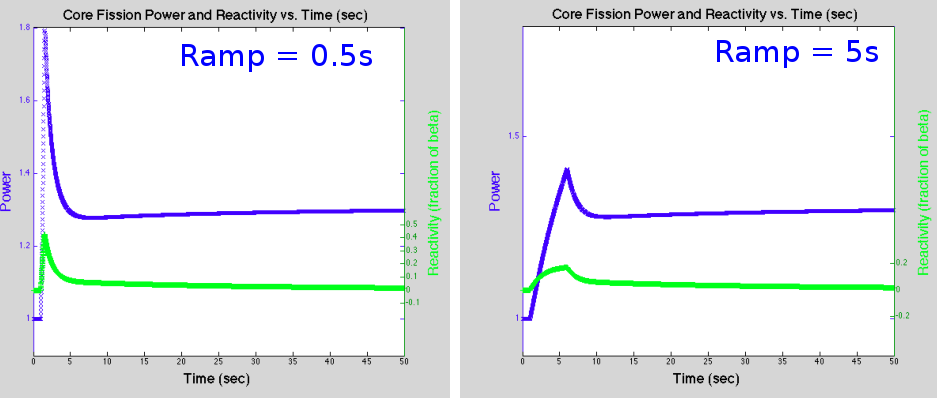
\includegraphics[width=6in]{images/pke/fn5.png}
  \caption{$0.5 \beta$ Reactivity Change with Feedback}
\end{figure}

\item Ramp $-0.5\beta$ reactivity. Undershoots are very common in negative reactivity transients. The slower ramping results in smaller $\Delta \rho, \Delta P$ because slow transients are in pseudo-equilibrium, and there is enough time for the feedback. That is, \textbf{The smaller rate of reactivity change is, the smaller the overshoot/undershoot is.} The final/asymptotic results are a different story, as they only depend on $\Delta \rho$ (system always find stable points) and are independent of $\drhodt$. 

\begin{figure}[ht]
  \centering
  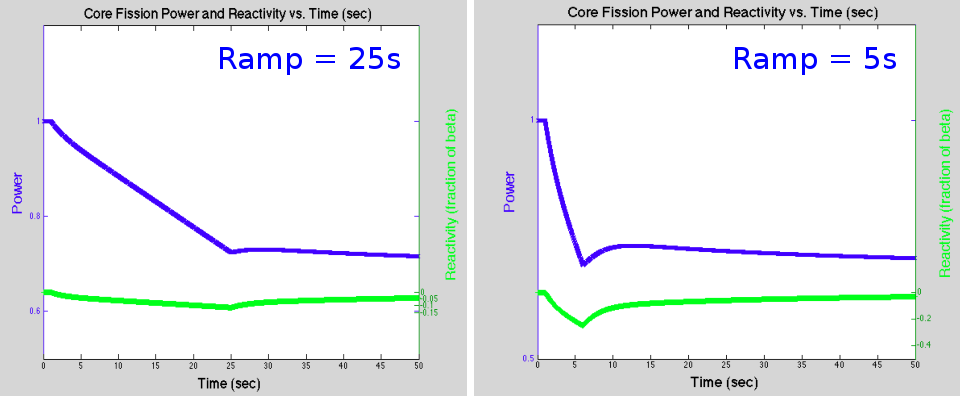
\includegraphics[width=6in]{images/pke/fn6.png}
  \caption{$-0.5 \beta$ Reactivity Change with Feedback}
\end{figure}

%Selective ramp insertion: 2 sec, power comes down quickly and recoveries, the radial heat gets high, close to an DNDF failure, makes sure to take into account the power rise. 

\clearpage
\item 1.5 $\beta$ RIA from HZP(eject rod in 0.1s, scram delay = 0.5s, scram time = 1s, follow to 3s). Nominal rated power increases by about 100 times in 0.2s. The power and temperature turns around due to Doppler feedback. Temperature peaks around 800K and ends around 760K: 
  \eqn{ T_{\mathrm{fuel}}^{\mathrm{end}} = \frac{2 (1.5 \times 0.0066 - 0.0066)}{3 \times 10^{-5}} + 540 = 761 \K} 

\begin{figure}[ht]
  \centering
  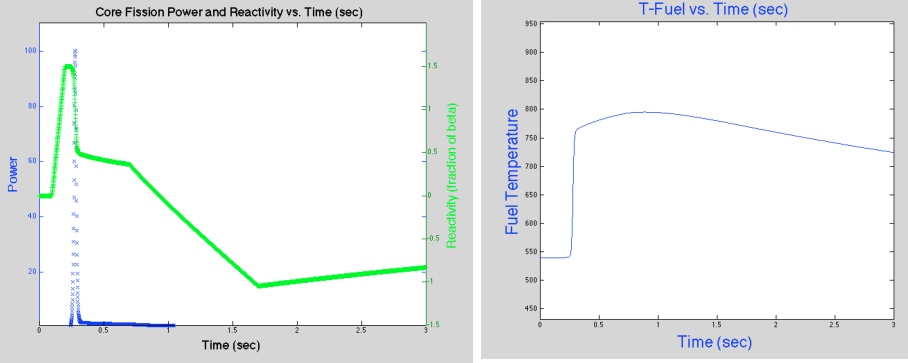
\includegraphics[width=6in]{images/pke/fn7.png}
  \caption{$1.5\beta$ RIA from HZP with Feedback}
\end{figure}


\item 1.5 $\beta$ RIA from HFP (exact same condition as last one except HFP this time). Power increases by about 70 times. Because we start at a higher power region, we get feedback more quickly, thus peak power is lower compare with the HZP case. $\Delta T$ is about the same as the HZP (initial temperature is higher, peak fuel temperature around 1200K) because the $\Delta \rho$ are the same for the two cases and our Doppler feedback coefficient is linear. 
\begin{figure}[ht]
  \centering
  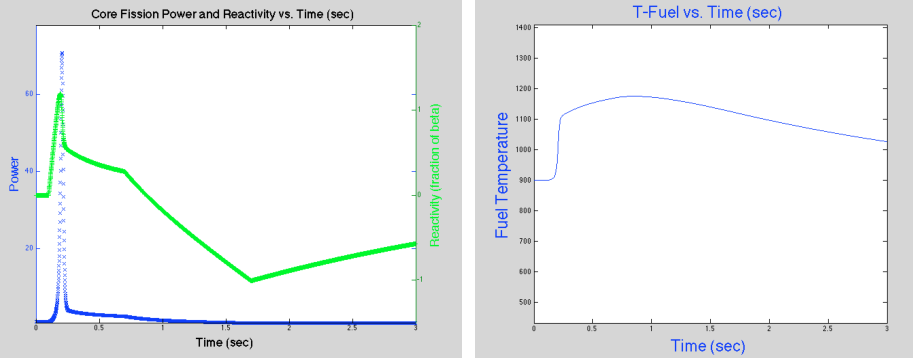
\includegraphics[width=6in]{images/pke/fn8.png}
  \caption{$1.5\beta$ RIA from HFP with Feedback}
\end{figure}

\clearpage
\item 1.5 $\beta$ RIA from HZP (same condition as the previous HZP RIA case, but eject rod in 1s instead of 0.1s). Power only goes up by 4 times in 1s. Again Doppler feedback turns the power around, and temperature peaks around 800K which is the same as  the fast ejection case. 

\begin{figure}[ht]
  \centering
  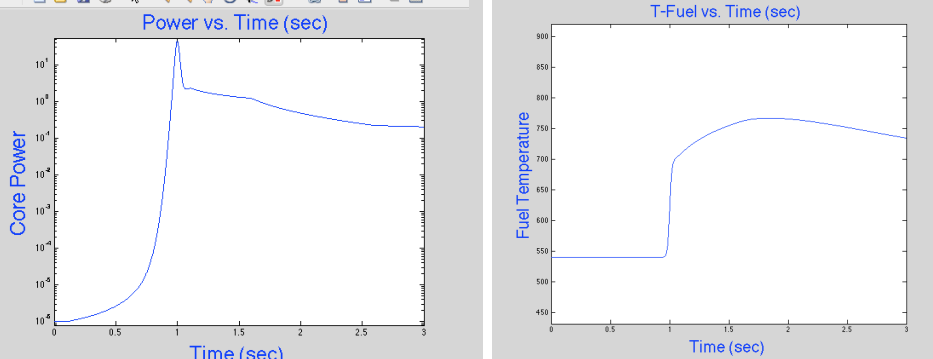
\includegraphics[width=6in]{images/pke/fn9.png}
  \caption{$1.5\beta$ RIA from HZP with Feedback, Slower Ejection}
\end{figure}


\item $1.5 \beta$ RIA from HFP (same condition as the previous HFP RIA case, but eject rod in 1s instead of 0.1s). The ejection is slow enough that the reactor is at equilibrium the whole time. The power peaks by a factor of 5 in 0.2s. Peak fuel temperature is around 1200K which is again the same as the fast ejection case. 

\begin{figure}[ht]
  \centering
  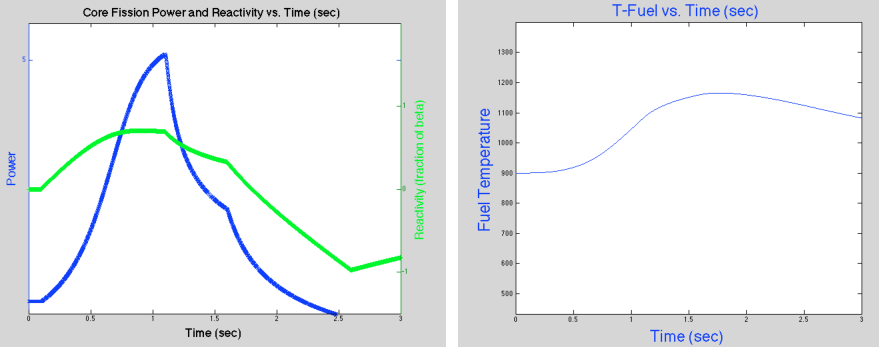
\includegraphics[width=6in]{images/pke/fn10.png}
  \caption{$1.5\beta$ RIA from HFP with Feedback, Slower Ejection}
\end{figure}

\clearpage
\item $1.5 \beta$ bank withdrawal RIA from HZP (eject in 100s). The ejection is so slow that the reactor is at equilibrium the whole time and the system never get super prompt critical (Doppler stops power ascension). The system reaches its nominal rated power in 100s. 

\begin{figure}[ht]
  \centering
  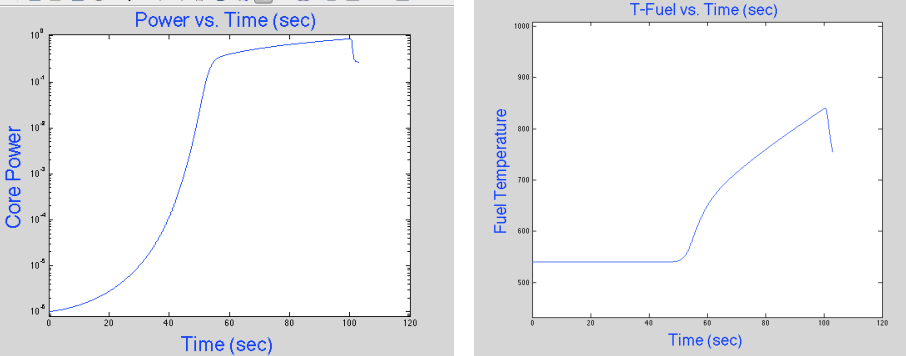
\includegraphics[width=6in]{images/pke/fn11.png}
  \caption{$1.5\beta$ RIA from HZP with Feedback, Slowest Ejection}
\end{figure}

\item $1.5 \beta$ bank withdrawal RIA from HFP (eject in 100s). Doppler reactivity is continually synchronized with rod reactivity (hence the straight line looking?). The system reaches twice its nominal rated power in 100s. 

\begin{figure}[ht]
  \centering
  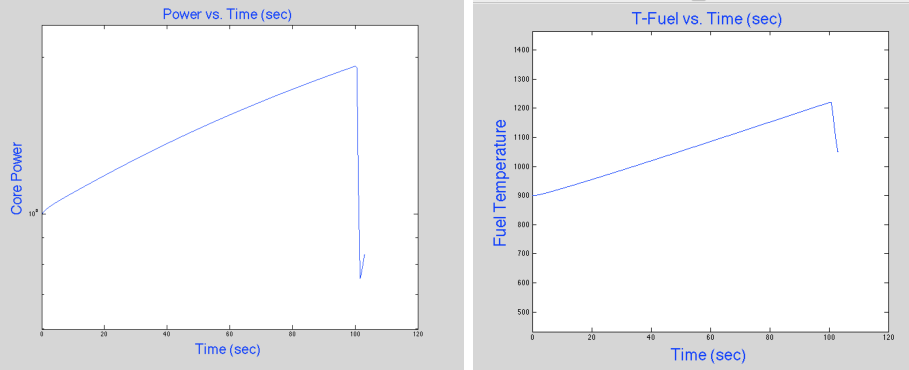
\includegraphics[width=6in]{images/pke/fn12.png}
  \caption{$1.5\beta$ RIA from HFP with Feedback, Slowest Ejection}
\end{figure}


\clearpage
\item $1.5 \beta$ bank withdrawal RIA from HFP (eject in 100s, no scram). Doppler reactivity is continually synchronized with rod reactivity (hence the straight line looking?). The ejection is slow enough that if we can take away the scram, and the system reaches a new equilibrium at twice its nominal rated power in 100s. 

\begin{figure}[ht]
  \centering
  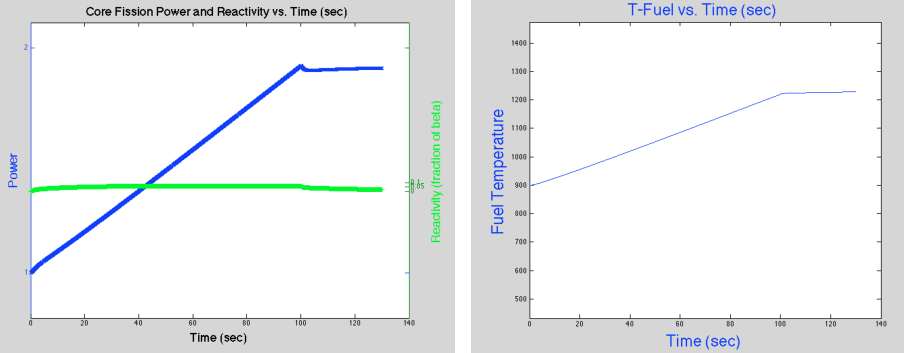
\includegraphics[width=6in]{images/pke/fn13.png}
  \caption{$1.5\beta$ RIA from HFP with Feedback, Slowest Ejection, No Scram}
\end{figure}
\end{enumerate}
Take-away: we don't really care about the temperal difference/integration, because the asymptotic temperature only depends on the reactivity change, not on the time dependent behavior. 



\clearpage
\topic{Summary}
\begin{enumerate}
\item PKEs assume you are solving for the core average properties; PKEs assume flux spatial shape is constant. Thus PKEs are not very precise for large spatial flux changes. 
\item Peak temperature are proportionally larger than core average properties.
\item If we really want spatial dynamics, we need to do 3D spatial dynamics to get correct predictions to complicated problems. 
\end{enumerate}
This thermal hydraulics model we have is very crude. For one thing, it has a huge diffusive property, that is, it would not predict any thermal shock behavior. 


%%%%%%%%%%%%%%%
As in Fig.~\ref{fn4}, about 3\% of the energy deposited into the coolant (about $2.5 \times 2$ MeV $=$5 MeV worth of neutrons from 200 MeV just from neutron slowing down that is deposited into the coolant), hence the coolant temperature would change slightly as well. Net reactivity comes back to zero. Remember \hi{PKEs are not precise for large spatial flux changes.}
  \begin{figure}[ht] 
    \centering
    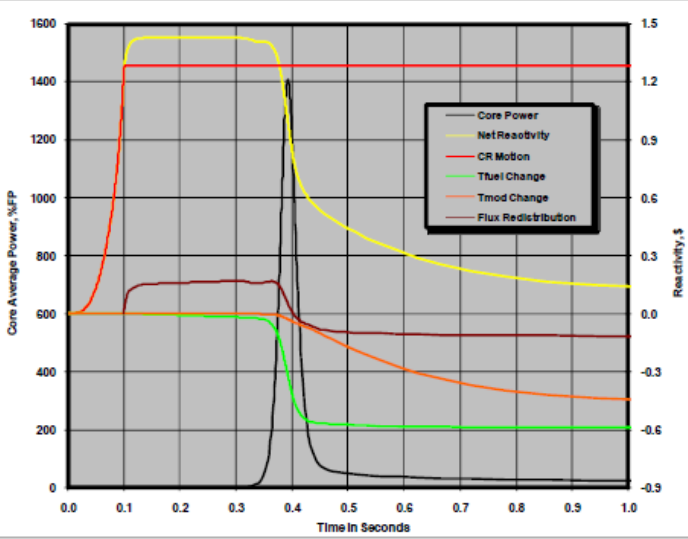
\includegraphics[width=6in]{images/pke/fn4.png}
    \caption{PWR Reactivity Insertion Accident} \label{fn4}
  \end{figure}


\end{document}
